\documentclass[10pt,fleqn,draft]{article} % Default font size and left-justified equations
\usepackage[%
    pdftitle={Contacts et mobilités},
    pdfauthor={Geoffrey Vaquette}]{hyperref}
    \usepackage{import}
\subimport{../../../../style/}{preambule.tex}
\usepackage{subcaption}

%\fichetrue
\fichefalse
\proftrue
%\proffalse
%\tdtrue
\tdfalse
\courstrue
%\coursfalse
\subimport{../../../../style/}{new_style}
\subimport{../../../../style/}{macros_SII}
\subimport{../../../../style/}{preambule_trou.tex}

\usepackage{siunitx}
% -------------------------------------
% Déclaration des titres
% -------------------------------------

\def\discipline{Enseignement \\Technologique \\ Transversal}
\def\xxtete{Enseignement Technologique Transversal}

\def\classe{1 STI2D}
\def\xxnumpartie{Seq 4}
\def\xxpartie{Modéliser les interactions entre solides}

\def\xxnumchapitre{Séance 1}
\def\xxchapitre{\hspace{.12cm} Contacts et mobilités}

\def\xxposongletx{2}
\def\xxposonglettext{1.45}
\def\xxposonglety{23}
\def\xxonglet{Seq. 4 -- Se. 1}

\def\xxactivite{Cours}
\def\xxauteur{\textsl{Geoffrey Vaquette}}

\def\xxcompetences{%
\textsl{%
\textbf{Compétences visées :}
\begin{itemize}[label=\ding{112},font=\color{ocre}]
\item \textbf{CO5.1} Expliquer des éléments d’une modélisation proposée relative au comportement de tout ou partie d’un système
\item \textbf{CO5.2} Identifier des variables internes et externes utiles à une modélisation, simuler et valider le comportement du modèle
\end{itemize}
\textbf{Connaissances abordées dans ce cours : }
\begin{itemize}[label=\ding{112},font=\color{ocre}]
\item 3.1.2 Typologie des solutions constructives des liaisons entre solides
\begin{itemize}
  \item Caractérisation des liaisons sur les systèmes
\end{itemize}
\end{itemize}
%
}}

\def\xxfigures{
\begin{center}
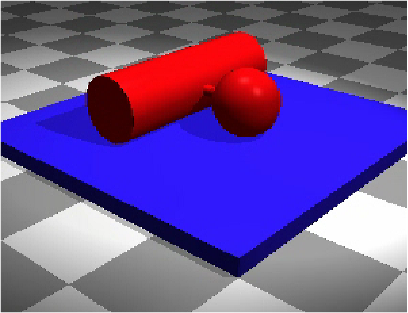
\includegraphics[width=3cm]{images/lineique_ponctuel} \\
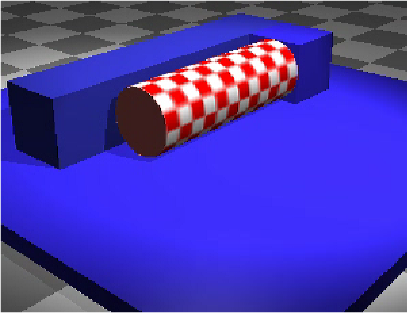
\includegraphics[width=3cm]{images/2lineique_1ponctuel} \\
% 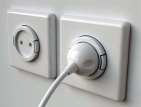
\includegraphics[width=2cm]{images/prise.png} \\
\end{center}
}%figues de la page de garde
\def\xxpied{%
La fonction alimenter/stocker \xxactivite%
}

%---------------------------------------------------------------------------

\renewcommand{\RemplirTrou}{true}
\begin{document}
\chapterimage{images/bandeau.jpg}
\subimport{../../../../style/}{new_pagegarde}
\section*{Introduction}
\paragraph{Solides parfaits}
\begin{itemize}
    \item Géométrie parfaite.
    \begin{itemize}
        \item Solides rigides (distance entre 2 points quelconque invariante au cours du temps).
        \item Solides indéformables (forme invariable quelque soient les sollicitations imposées).
    \end{itemize}
\end{itemize}
On peut alors reconstituer la géométrie d'un solide à partir de volumes élémentaires (parallélépipède, cylindre, cône, tore, sphère).

\paragraph{Liaisons parfaites}
\begin{itemize}
    \item Pas de frottement
    \item Géométrie des contacts parfaite
\end{itemize}
Pour modéliser l'interaction entre les pièces d'un produit, la première chose à observer est le type de contacts qu'il existe entre ces pièces.

\section{Degrés de liberté et degrés de liaison}
Dès qu'il y a contact entre deux solides, il y a alors
liaison entre ces solides. Les surfaces de contact suppriment des degrés de liberté et imposent des mobilités entre les deux solides.

On peut caractériser cette liaison soit :
\begin{itemize}
    \item à partir du type de contact
    \item à partir des mouvements relatifs des pièces.
\end{itemize}

Tout mouvement  relatif  entre  solides  liés  pourra  être  obtenu  par  une  combinaison de  ces  six  mouvements  de base.

\begin{itemize}
    \item Translation suivant x (notée \trou{Tx})
    \item Translation suivant y (notée \trou{Ty})
    \item Translation suivant z (notée \trou{Tz})
    \item Rotation suivant x (notée \trou{Rx})
    \item Rotation suivant y (notée \trou{Ry})
    \item Rotation suivant z (notée \trou{Rz})
\end{itemize}


\begin{defi}
\textbf{Degrés de liaison:}
C'est le nombre de déplacements élémentaires interdits par 
une liaison.

 \textbf{ Degrés  de  liberté  d'une  liaison:}
  
\trou{C'est  le  nombre  de  déplacements  élémentaires 
indépendants autorisés par cette liaison.}

La somme des degrés de liberté et des degrés de liaison est égale à : \trou{6}. 
En effet, les degrés non bloqués sont tous des degrés de liberté et inversement. 
\end{defi}
rpcinematik

\begin{exemple}
  A partir de cette image et des indications, on peut déterminer les nombres de \begin{itemize}
        \item degrés de liaison : \trou{5}
        \item degrés de liberté : \trou{1}
        \item Somme : \trou{5+1=6}
  \end{itemize}
\end{exemple}


\section{Différents types de contacts}
\begin{aretenir}
  À l'aide des différentes formes de la Figure~\ref{fig:volumes}, on peut définir trois types de contacts : les contacts \trou{surfaciques}, \trou{linéiques} et \trou{ponctuels}.
\end{aretenir}

\begin{remark}
  Pour mettre en évidence ces contacts, on peut imaginer plonger une des pièces dans de la peinture, mettre en contact les deux pièces puis observer la trace laissée sur la pièce non peinte.
\end{remark}

Un exemple de chaque type de contact est donné sur la Figure~\ref{fig:type_contact}.

\begin{figure}[h]
  \begin{subfigure}[b]{0.3\textwidth}
    \centering
    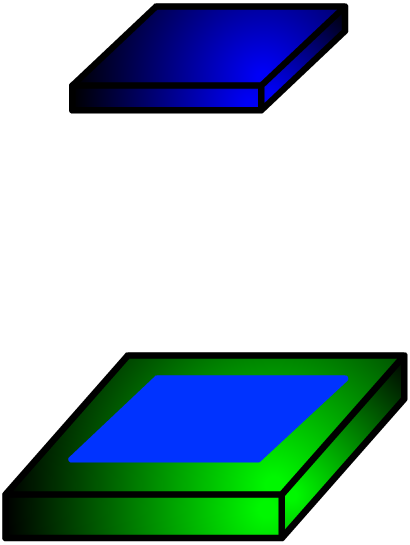
\includegraphics[width=0.9\textwidth,height=.2\textheight,keepaspectratio]{images/plan-plan}
    \caption{\trou{Contact surfacique}}
  \end{subfigure}\hfill
  \begin{subfigure}[b]{0.3\textwidth}
    \centering
    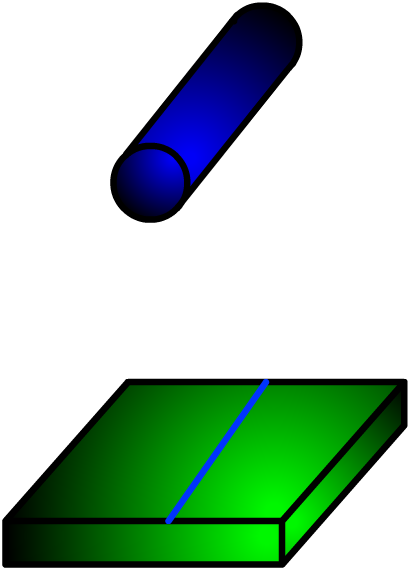
\includegraphics[width=0.9\textwidth,height=.2\textheight,keepaspectratio]{images/cylindre-plan}
    \caption{\trou{Contact linéique}}
  \end{subfigure}\hfill
  \begin{subfigure}[b]{0.3\textwidth}
    \centering
    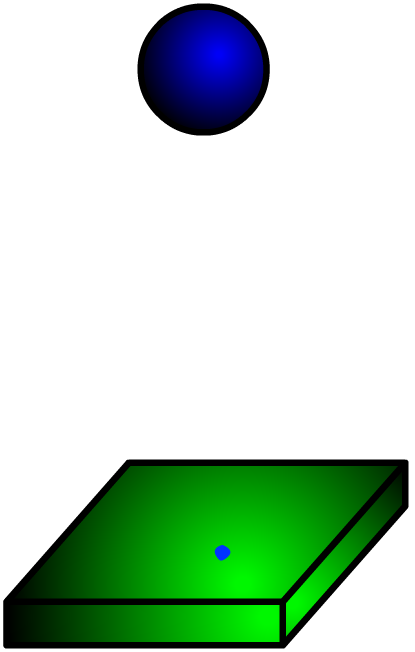
\includegraphics[width=0.9\textwidth,height=.2\textheight,keepaspectratio]{images/sphere-plan}
    \caption{\trou{Contact ponctuel}}
  \end{subfigure}\hfill
  \caption{Un exemple de chaque type de contact}
  \label{fig:type_contact}
\end{figure}
\subsection{Les contacts surfaciques}

\begin{defi}
  On dit qu'un contact est surfacique lorsque la zone de contact entre deux pièces est une surface non nulle (on peut calculer l'air de cette surface).
\end{defi}

\begin{warn}
  Une surface n'est pas forcément plane (plate).
\end{warn}

Dans ce cours, nous retiendrons trois types de contacts surfaciques, représentés sur la Figure~\ref{fig:surfacique}

\begin{figure}[h]
  \begin{subfigure}[b]{0.3\textwidth}
    \centering
    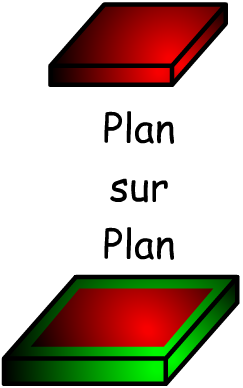
\includegraphics[width=0.9\textwidth,height=.15\textheight,keepaspectratio]{images/surface_plan}
    \caption{Plan sur plan}
  \end{subfigure}\hfill
  \begin{subfigure}[b]{0.3\textwidth}
    \centering
    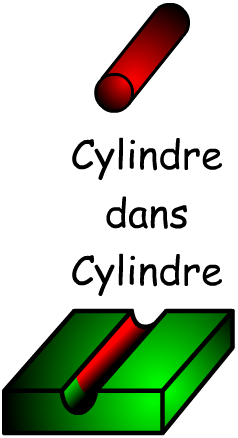
\includegraphics[width=0.9\textwidth,height=.15\textheight,keepaspectratio]{images/surface_cylindre}
    \caption{Cylindre sur plan}
  \end{subfigure}\hfill
  \begin{subfigure}[b]{0.3\textwidth}
    \centering
    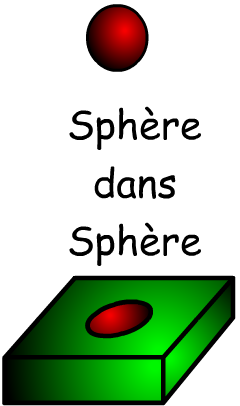
\includegraphics[width=0.9\textwidth,height=.15\textheight,keepaspectratio]{images/surface_sphere}
    \caption{Sphère dans sphère}
  \end{subfigure}\hfill
  \caption{Trois types de contacts surfaciques}
  \label{fig:surfacique}
\end{figure}

\subsection{Contacts linéiques}
\begin{defi}
  On dit qu'un contact est linéique lorsque la zone de contact entre deux pièces est une ligne. Cette ligne peut être \trou{rectiligne} (une droite) ou \trou{annulaire} (circulaire).
\end{defi}

\begin{figure}[h]
  \begin{subfigure}[b]{0.5\textwidth}
    \centering
    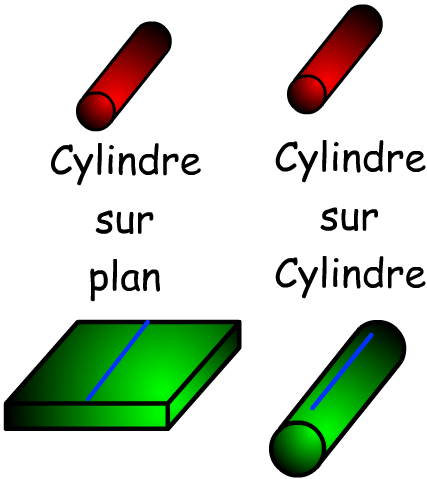
\includegraphics[width=0.9\textwidth,height=.2\textheight,keepaspectratio]{images/lineaire_rectiligne}
    \caption{Contact linéaire \trou{rectiligne}}
  \end{subfigure}\hfill
  \begin{subfigure}[b]{0.5\textwidth}
    \centering
    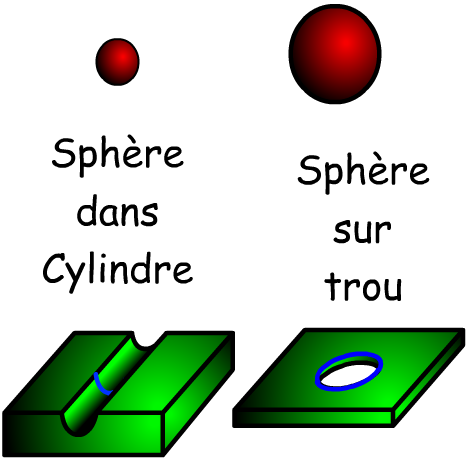
\includegraphics[width=0.9\textwidth,height=.2\textheight,keepaspectratio]{images/lineaire_annulaire}
    \caption{Contact linéaire \trou{annulaire}}
  \end{subfigure}\hfill
  \caption{Contacts linéiques}
  \label{fig:surfacique}
\end{figure}

  \subsection{Les contacts ponctuels}
  \begin{defi}
    On dit qu'un contact est ponctuel lorsque la zone de contact entre deux pièces est un point.
  \end{defi}
\begin{figure}[h]
  \centering
  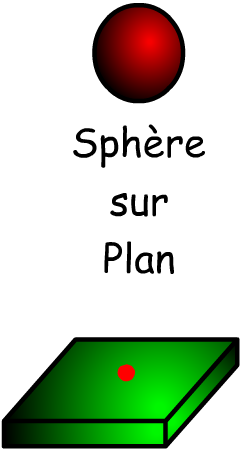
\includegraphics[width=0.9\textwidth,height=.2\textheight,keepaspectratio]{images/ponctuel}
  \caption{Contact ponctuel}
  \label{fig:ponctuel}
\end{figure}
\pagebreak
\section{Exemples de contacts entre pièces}
\begin{exemple}
  Prenons l'exemple de la pièce en Figure~\ref{fig:exemple1}, la pièce rouge a deux contacts avec la pièce bleu. Ces contacts sont :

  \begin{itemize}
    \item Un contact \trou{linéique rectiligne}
    \item Un contact \trou{ponctuel}
  \end{itemize}
\end{exemple}
\begin{figure}[h]
  \centering
  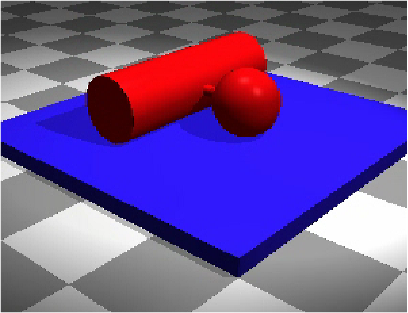
\includegraphics[width=0.9\textwidth,height=.2\textheight,keepaspectratio]{images/lineique_ponctuel}
  \caption{Exemple 1}
  \label{fig:exemple1}
\end{figure}

\begin{exemple}
  Prenons l'exemple de la pièce en Figure~\ref{fig:exemple2}, la pièce rouge a \trou{trois} contacts avec la pièce bleu. Ces contacts sont :

  \begin{itemize}
    \item \trou{Deux contacts linéiques rectilignes}
    \item \trou{Un contact ponctuel}
  \end{itemize}
\end{exemple}
\begin{figure}[h]
  \centering
  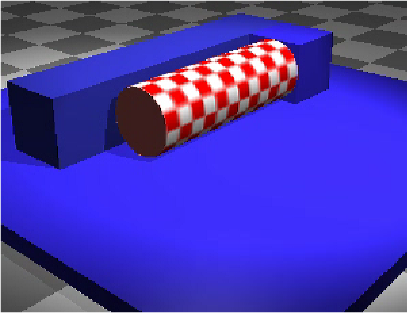
\includegraphics[width=0.9\textwidth,height=.2\textheight,keepaspectratio]{images/2lineique_1ponctuel}
  \caption{Exemple 2}
  \label{fig:exemple2}
\end{figure}

\begin{remark}
  Les exercices utilisés durant cette séance sont tirés du site suivant. Vous trouverez sur cette page des exercices pour vous entrainer à reconnaître les contacts entre pièces.\\
  \url{http://www.ecligne.net/mecanique/1_modelisation/1_les_contacts/sommaire.html}
\end{remark}

\end{document}
